% Chapter 3

\chapter{System Overview} % Main chapter title

\label{systemoverview} % For referencing the chapter elsewhere, use \ref{Chapter1} 

\lhead{Chapter 3. \emph{System Overview}} % This is for the header on each page - perhaps a shortened title

%----------------------------------------------------------------------------------------

\section{Introduction}

The Context-Aware Guide (subsequently called "CA Guide" or simply "Guide") needs to be defined to fit indoor, outdoor and mixed sites, like classical museums, parks and gardens. 
The basic functionality must be accessible even by persons not familiar with mobile technology. The context awareness techniques can help avoiding big parts of explicit user input, allowing the visitor to focus completely on it's environment without reading and typing numbers.

This thesis, however, focuses on the technical foundation of the whole system, and thus on the system architecture on several levels of abstraction. 

The following figure shows a high level view of the complete system, consisting of the visitor guide front-end running on a mobile device, a back-end for the modelling the guide and performing analytic functions. The database server is accessed by both system parts and represents the communication basis - there is no direct communication between font and back end. All data is exchanged over the database, enabling asynchronous communication.

As database server Couchbase was chosen due to it's automatic synchronization capabilities, it's mobile version and it's ability to scale out without completely redesigning the way the database is accessed by the application.\footnote{After actually having reached the limits of scalability of a single classical relational database server in a commercial project and painfully distributing the database on several servers of the productive system, the idea of an easy scale out using a NoSql database cluster and map-reduce queries seems very attractive to me.} 

\begin{figure}[H]
\centering
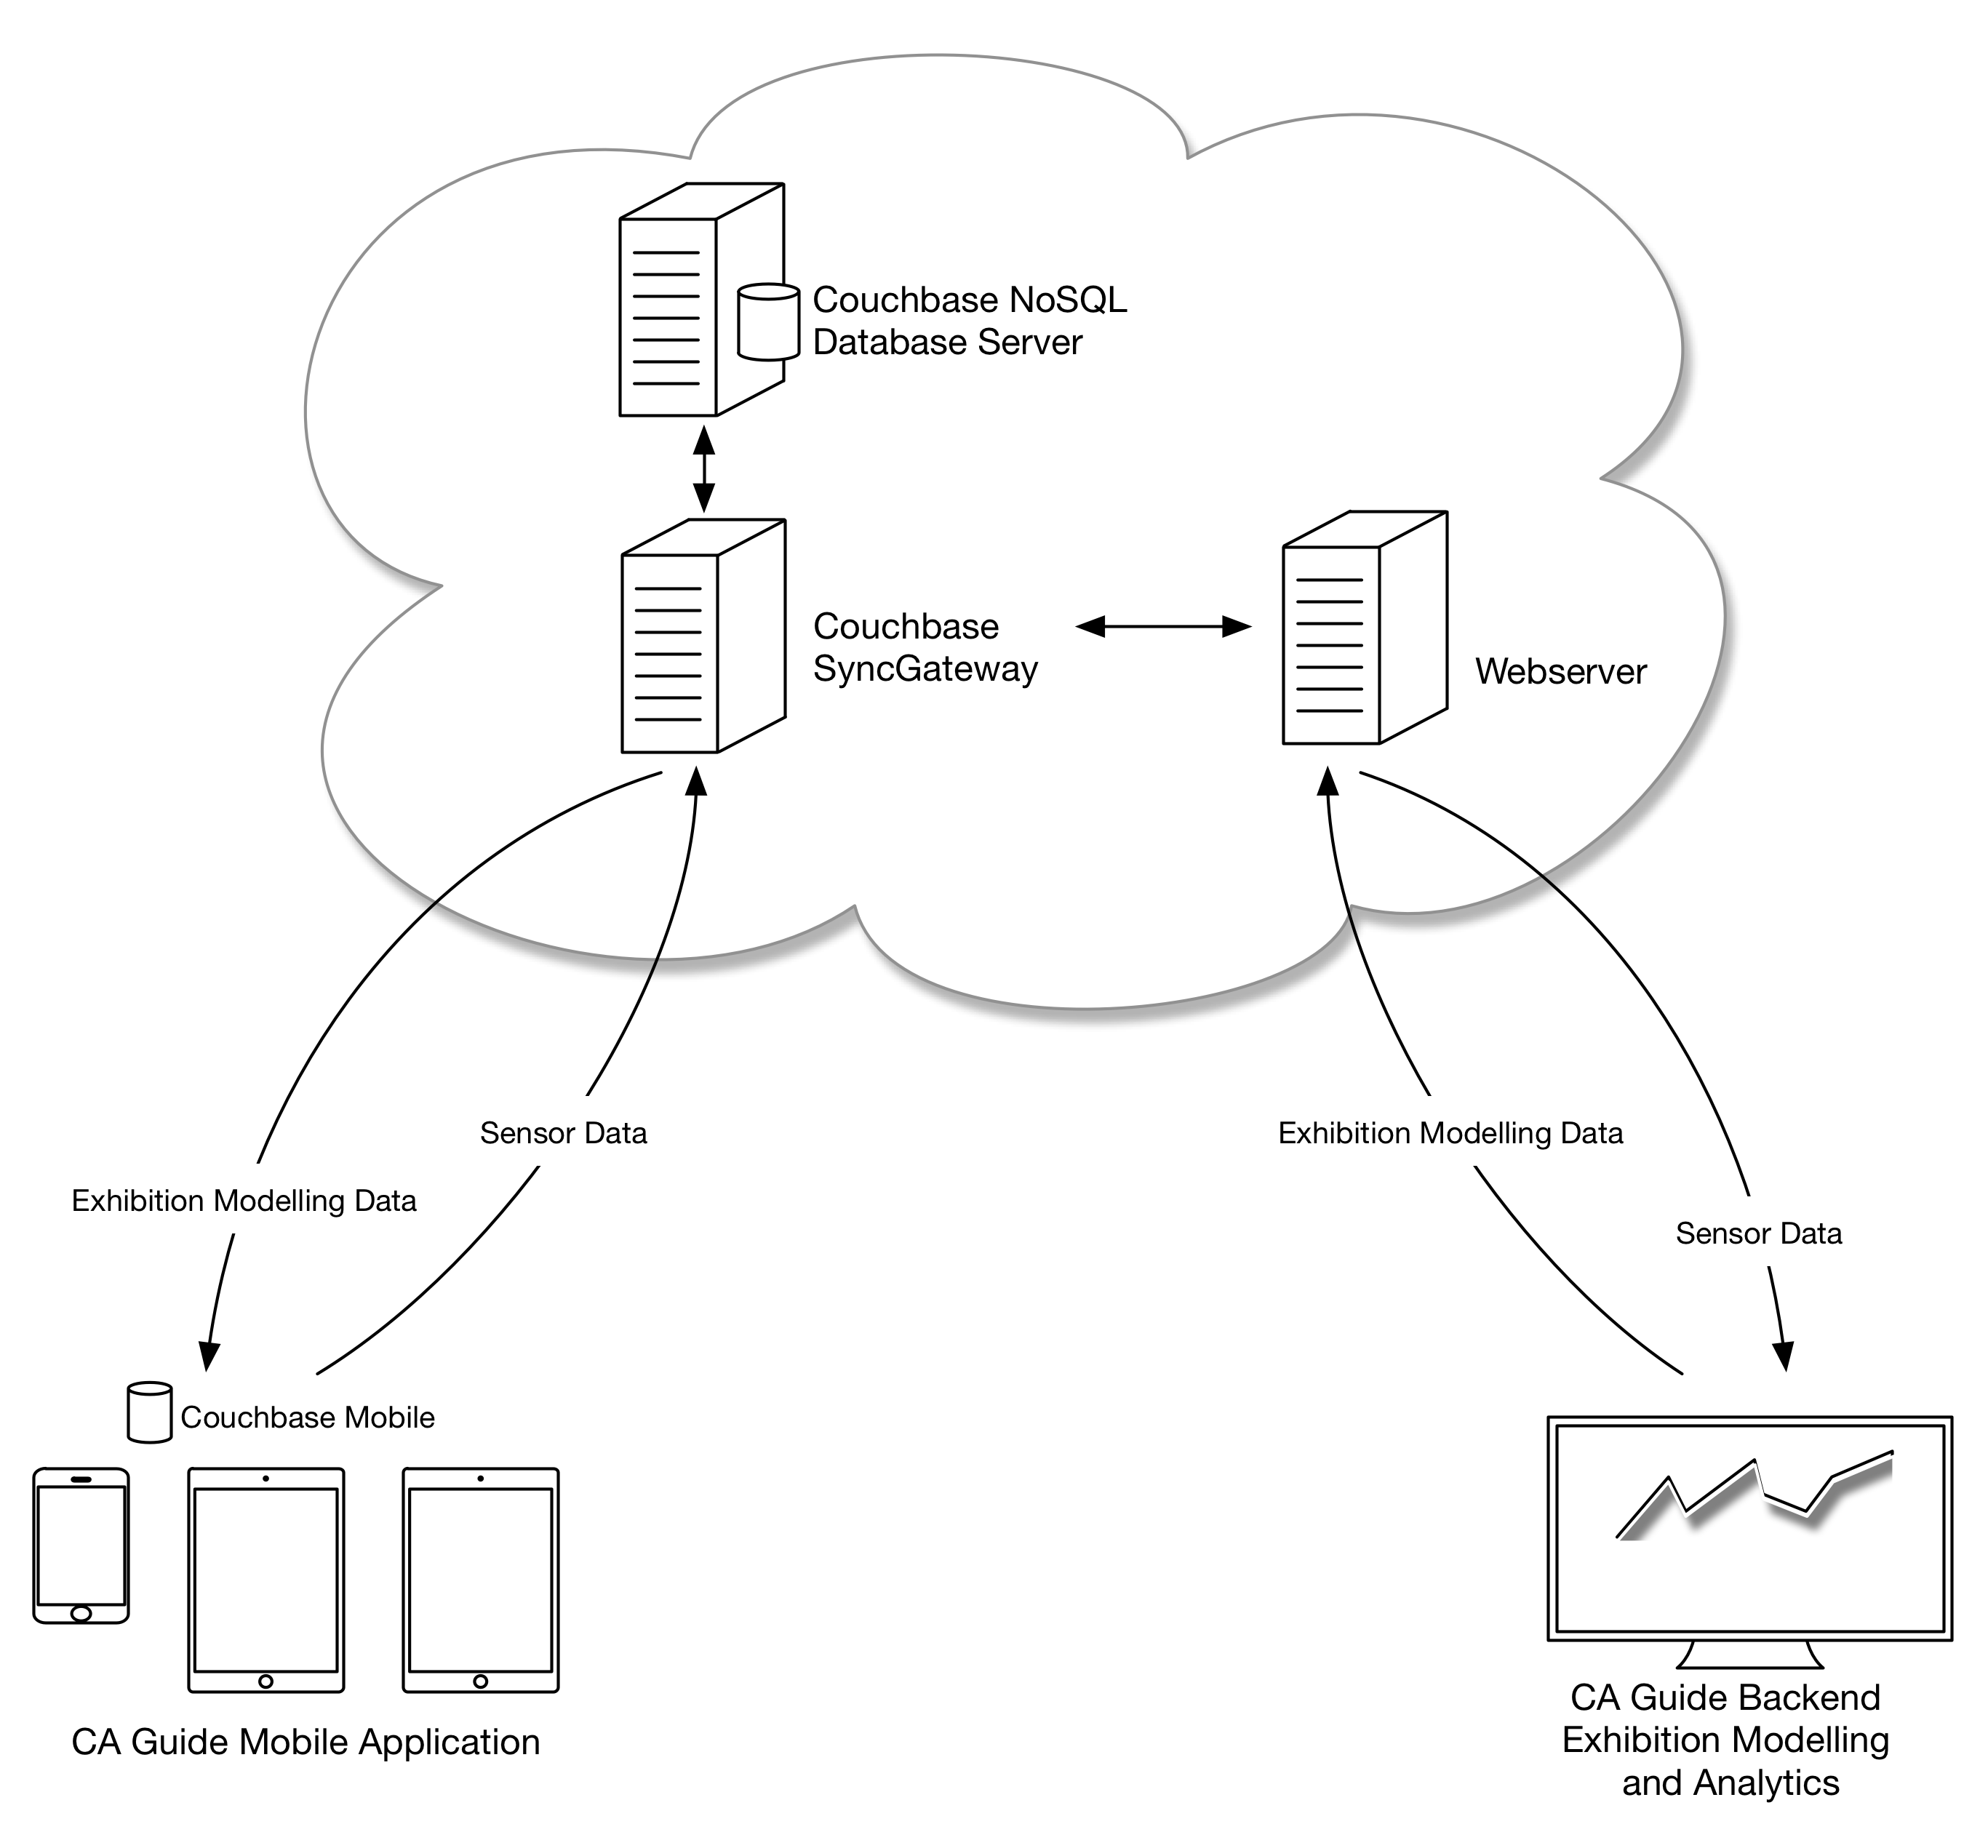
\includegraphics[height=0.8\textwidth]{system-overview}
\caption{CA Guite Architecture Overview}
\end{figure}

%Image Mockup CA Guide 
%Image A Backend Screen Mockup

The two system parts share a unique data structure for the site model containing all data needed for the mobile guide and the sensor traces, containing recorded raw or computed measurements at different time intervals. Thus, before starting with the front or back-end, it is important to reason about the common data model.

\section{Data Model}

\subsection{Site Modelling}

A single park or museum is modeled using the JSON data format. Compared to XML, JSON is more readable, easier to produce without dedicated tools in a simple text editor and more compact, mainly on account of the elimination of duplicated entity names in closing tags.

The main entities used for modeling a site are shown on the following picture.

\begin{figure}[H]
\centering
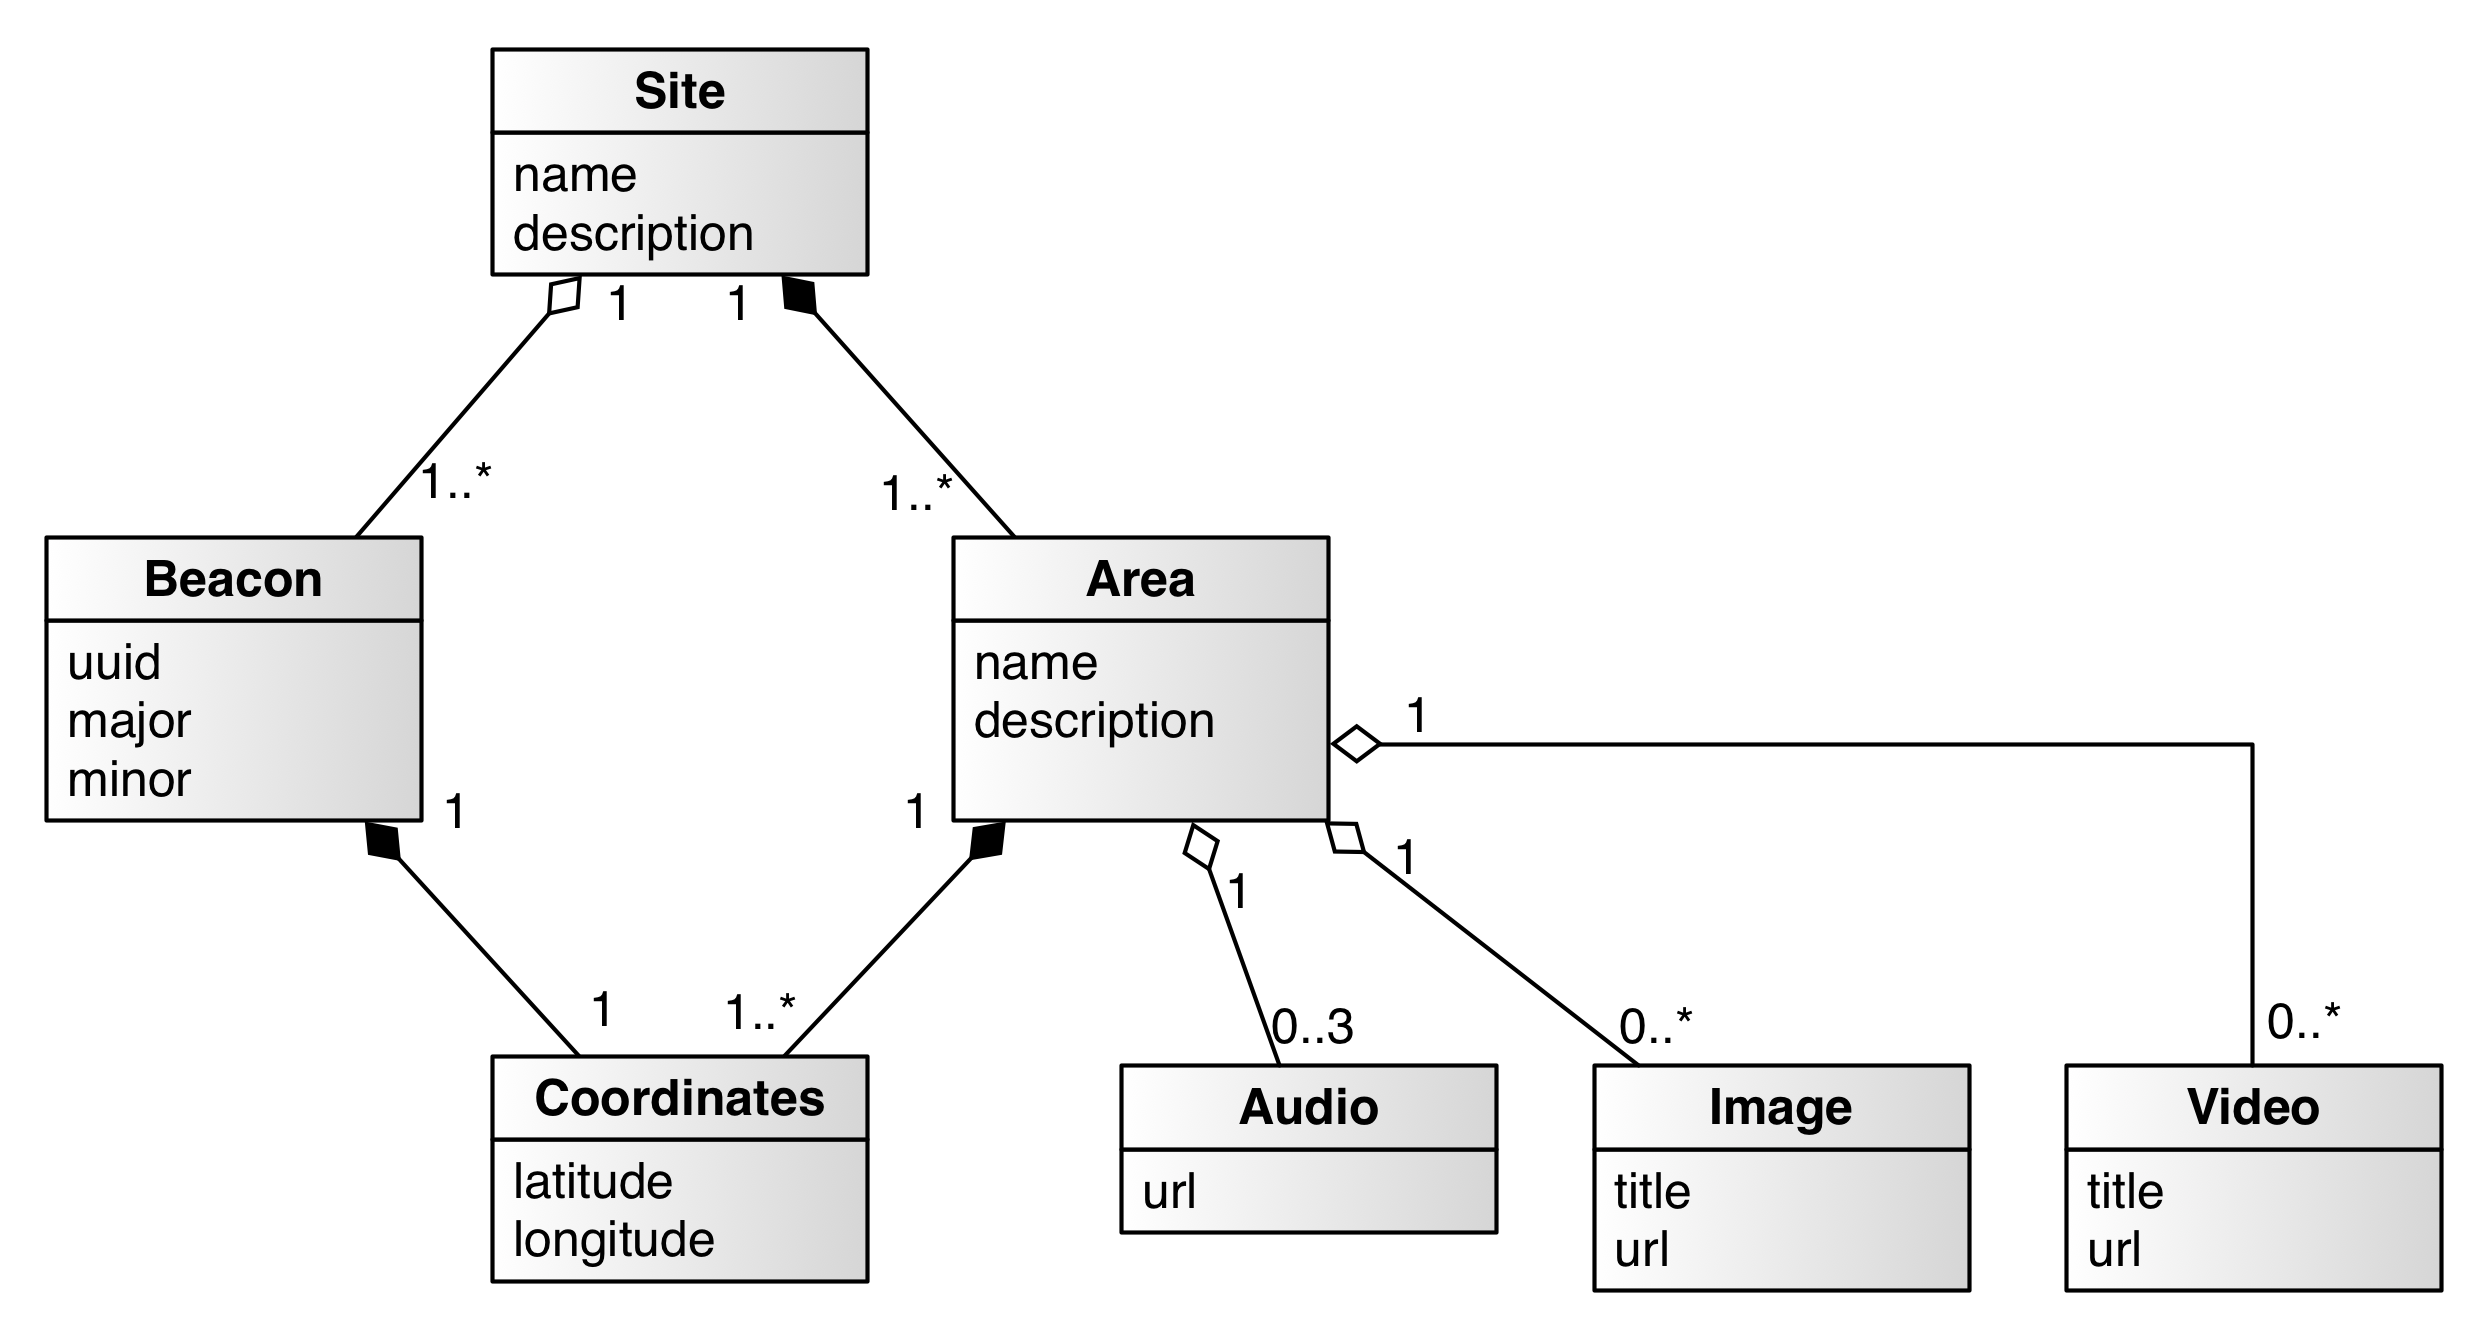
\includegraphics[height=0.5\textwidth]{data-model-site}
\caption{Data model of a site (using UML notation)}
\end{figure}

A site is composed of several areas, geographically delimited by a list of coordinates. For indoor sites, several beacons can be added with their identifying properties and the defined position. Beacons are decoupled from areas in the data model. They are a positioning help\footnote{After the mobile front-end determined it's (indoor) position based on the beacon's data, it identifies the area it is situated using geometrical computations} that could be replaced in the future.
An area has a textual description and optionally (even though in productive systems very likely) up to three audio files containing explanations as voice recordings and other fitting audio material. These three files reflect a rising level of detail. 
Furthermore, several images and videos can be added to the area.

With a normal relational database, pretty much of the entities would be saved in separate tables in a normalized way using primary and foreign keys to represent the relationships between the tables. In case of the one to many relation between an area and it's images, the usual way is to define a separate table "Image" and to store a title and the image or an url beside the areas id they belong to.

\begin{figure}[H]
\centering
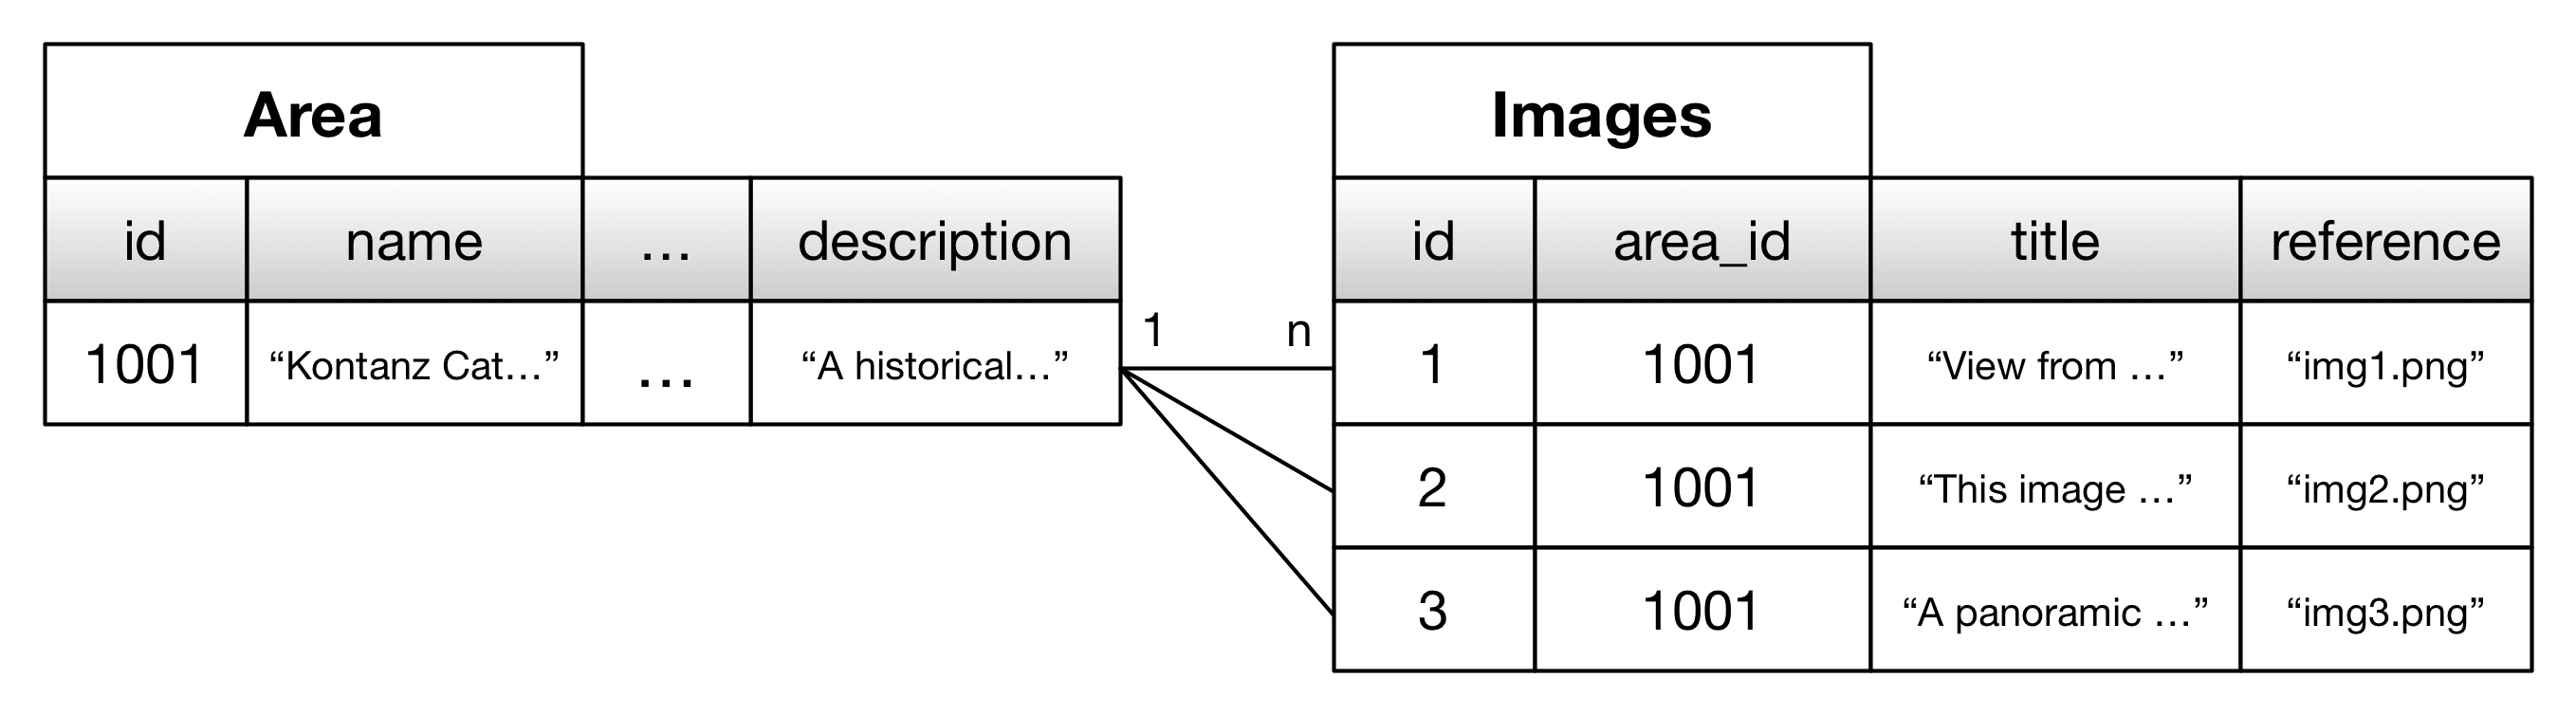
\includegraphics[width=0.7\textwidth]{relational-db-1n}
\caption{A 1:n relationship in a classical relational database}
\end{figure}

With a document-oriented database, data is commonly stored in a more aggregated way. In contrast to the records of a relational database, records of document-oriented database have a more complex structure allowing lists and nesting. In \cite{nosqldistilled}, the authors suggest the term "aggregate" for these type of records. They adopted this term from \cite{domaindriven} "Domain-Driven Design". An aggregate is a set of objects used together. That means they are loaded and saved to the database as a unit and they determine the unit to be locked for the management of consistency.  

So the precise level of aggregation depends mainly on how the data will be accessed later, and as is often the case, there is not only one right solution. 

From a site modeling point of view at the back-end, single areas and single beacons can be viewed as aggregates, allowing more granular modifications and enabling collaborative editing of a single site.
From a front-end point of view, a whole site definition can be regarded an aggregate. During initialization, the whole site is read with all areas and beacons. This can be done with a single database query. On the mobile device, sites are only read and never modified, so that there is no problem with a bigger aggregate that has to be locked.

Since having a working copy of a site for modeling in the back-end that is not deployed to the mobile devices until it is marked as finished is desirable, I decided to take a hybrid solution. On the back-end, a site is modeled with finer-grained aggregates having separate documents for sites, areas and beacons. These aggregates lies in a separate modeling database (or bucket, as they are called in Couchbase) that is not synchronized with the mobile devices.

At the point a the model is marked as finished, all these documents are merged into one big site aggregate, containing all the data. This document is written to the shared database and is automatically synchronized with the mobile databases as soon as they have networking connectivity. 

The site model can the be refined and edited at the back-end without compromising the deployed version. For productive usage, an additional shared testing database synchronized only with a testing mobile device would be necessary. The site aggregate could first be written to this database for testing before deploying it to the rest of the mobile devices. This functionality can be added at a later stage and is out of scope of this thesis.
 
The following JSON-document shows a simplified site aggregate containing one area with the simplest possible polygon and one beacon, to get an idea of the structure.

\begin{lstlisting}[basicstyle=\footnotesize,caption=An exemplary site aggregate in JSON representation]
key: "Site-CXN01"
value: {
 "type":"city",
 "name":"Konstanz",
 "description":"",
 "areas": [{
   "id":"area-51",
   "type":"area",
   "name":"Konstanz Cathedral", 
   "description":"A historical building in Konstanz, ...",
   "locationDefinition": {
	 "type": "polygon",
	 "coordinates": [
	   {"lat":47.663093, "lon":9.176371},
	   {"lat":47.663336, "lon":9.175215},
	   {"lat":47.663673, "lon":9.176075}]}, 
	 "images":["cathedral-panorama.png","cathedral-nw.png"], 
	 "audio":{
	   "level1": "cathedral-1.mp3",
	   "level2": "cathedral-2.mp3",
	   "level3": "cathedral-3.mp3"}, 
	 "videos":[]}],
 "beacons": [{
   "id":"beacon-42",
   "uuid":"F7826DA6-4FA2-4E98-8024-BC5B71E0893E",
   "major":"40231",
   "minor":"203",
   "coordinates": {"lat":47.663278, "lon":9.176214}}]
}
\end{lstlisting}

The binary data of images, audio files and videos can be stored outside of the document, maintaining only a reference to them inside the document (in this sample, a file name was used to represent a reference). Storing binary data outside of the document avoids wasting storage capacity due to inflation of data represented in a base64-encoded way and reduces the parsing time of the document.
For this purpose, Couchbase offers the concept of attachments, that can be associated to a document but are stored separately in a binary way. Another advantage is a higher efficiency of the replication, since attachments are not retransferred when the associated document was changed but only on real modifications of the attachment itself \cite{cbattachment}.

Although NoSQL databases are often referred to as being schema-less, it's important to keep in mind that there still is an implicit schema: the data structure the application relies on. The risk of malformed data can be handled with automated tests. Especially in case of manually produced JSON documents or JSON data coming from a foreign system, a JSON schema can be used for asserting a valid structure of a JSON file, similar to a DTD (Data Type Definition) in XML (http://json-schema.org).

\subsection{Sensor Data}

Sensor data measurements is saved to the Couchbase database to allow replaying it for development, testing, presentations and for analytics presented in the system's web back-end. Thus, the producer and consumer of the data is switched here, having the data produced inside the front-end, written into mobile database and later synchronized over the network with the Couchbase database for enabling read-only access by the back-end.  

\begin{figure}[H]
\centering
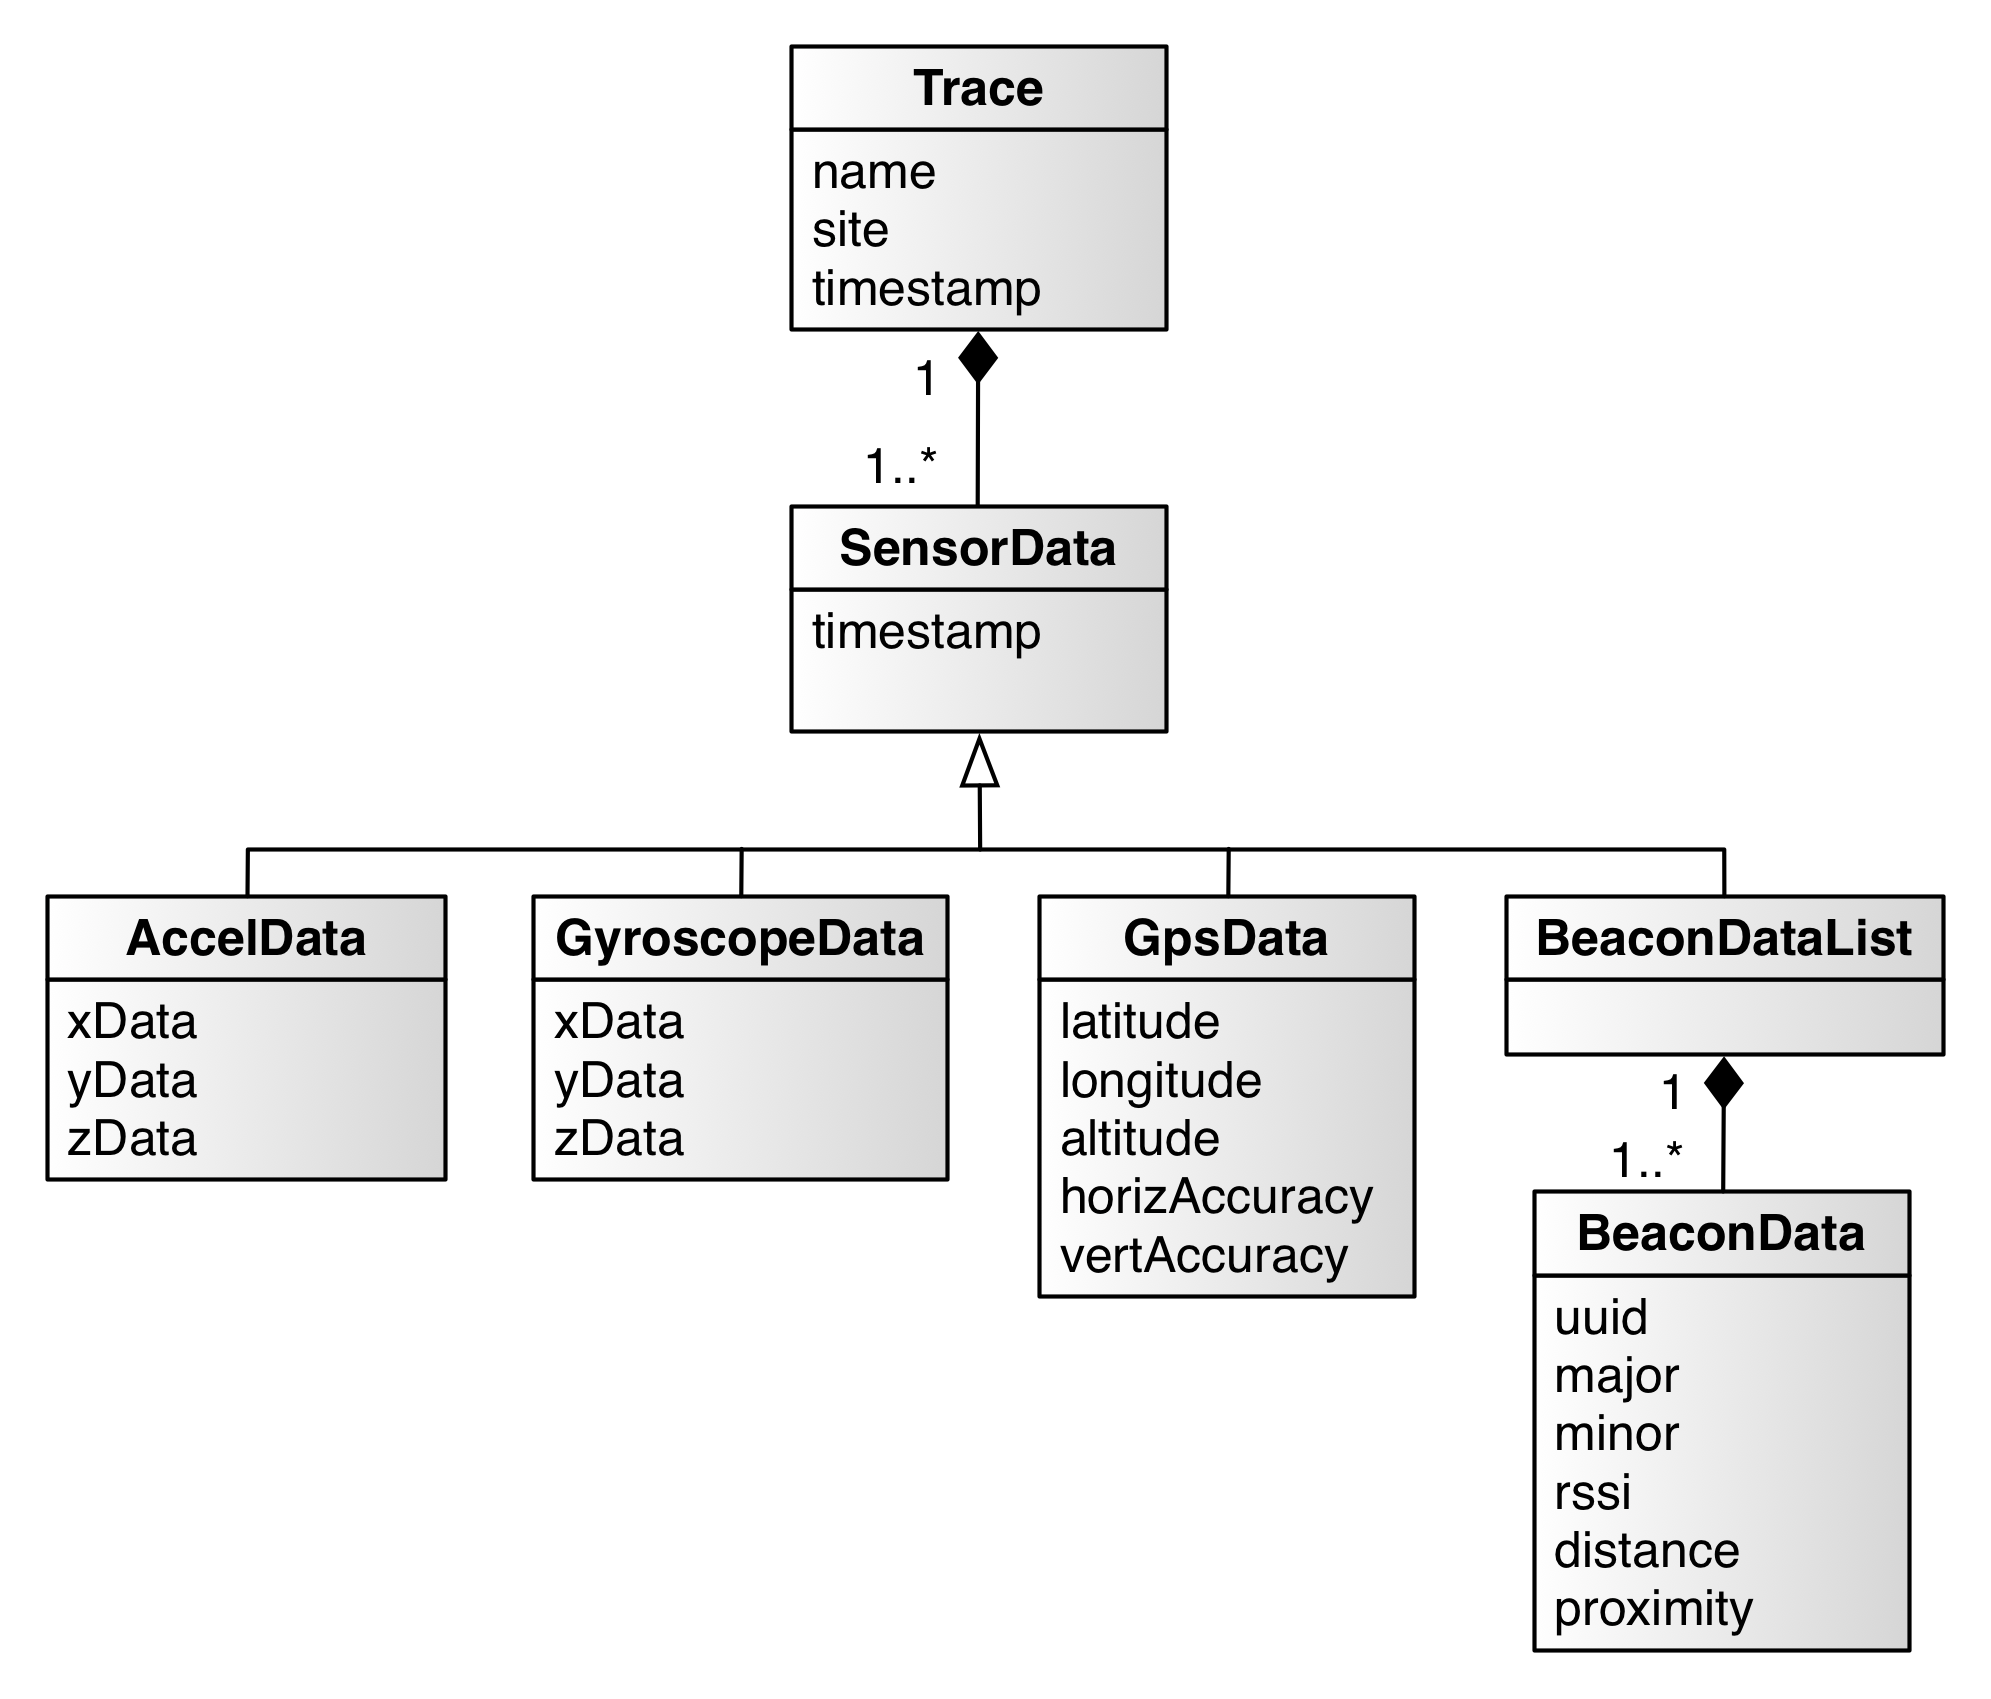
\includegraphics[height=0.5\textwidth]{data-model-trace}
\caption{Data model of a sensor trace}
\end{figure}

The single measurements can be very high frequent, for example in case of accelerometer data, that is updated every 10 milliseconds. Updates on beacon measurements and GPS measurements are typically available every second. Events on a higher logical level, like "entering region a", will occur much less frequently.

The two use cases are recording data for development and testing and recording visitor movements for analytics.
Low level testing sensor traces, containing 100 measurements per second for each sensor, will only be recorded over a limited time period for testing and profiling algorithms. 
The recording duration for analytic purposes during an actual visit can extend to hours, but at the same time only higher level data is recorded and thus the data amount grow much slower. Therefore, saving a trace into a single aggregate is considered feasible for both use cases.

The following listing shows a trace as JSON document with an exemplary sensor data measurement for each type.

\begin{lstlisting}[basicstyle=\footnotesize,caption=An exemplary trace aggregate in JSON representation]
key: Sensortrace-CXN01
value: {
  "type": "trace",
  "timestamp": 12345678.35,
  "site": "Site-CXN01",
  "data": [
    {"type":"accelerometer", "timestamp": 12345678.350, 
      "data": [1.235, 0.364, 0.021]},
    {"type":"gyroscope", "timestamp": 12345678.360, 
      "data": [0.031, 0.005, 0.207]},
    {"type":"gps", "timestamp": 12345678.495, "data": {
      "latitude":47.652712, "longitude":9.168142, "altitude":404.90, 
      "vertAccuracy":65, "horizAccuracy":10}
    {"type":"beacons", "timestamp": 12345678.782, "data": [
      {"uuid":"B9407F30-..6D", "major":14185, "minor":2, 
      	"proximity":1, "rssi":-67, "distance":0.53},
      {"uuid":"B9407F30-..6D", "major":14185, "minor":3, 
      	"proximity":2, "rssi":-77, "distance":4.53}    
    ]}
  ]
}
\end{lstlisting}


\section{Setting up the Couchbase Server Infrastructure}

After locally installing Couchbase Server, a web based admin console is accessible at http://localhost:8091. It offers an overview of the system status, performance details and several administration tasks. In case of having several servers attached, the whole cluster can be managed and analyzed over this web application.

For the guide platform, two Couchbase buckets are created: "guide" is the shared database and "guide-editor" the back-end only one. The following picture shows two screen shots of the cluster overview page and the data buckets page with our buckets.

\begin{figure}[H]
\centering
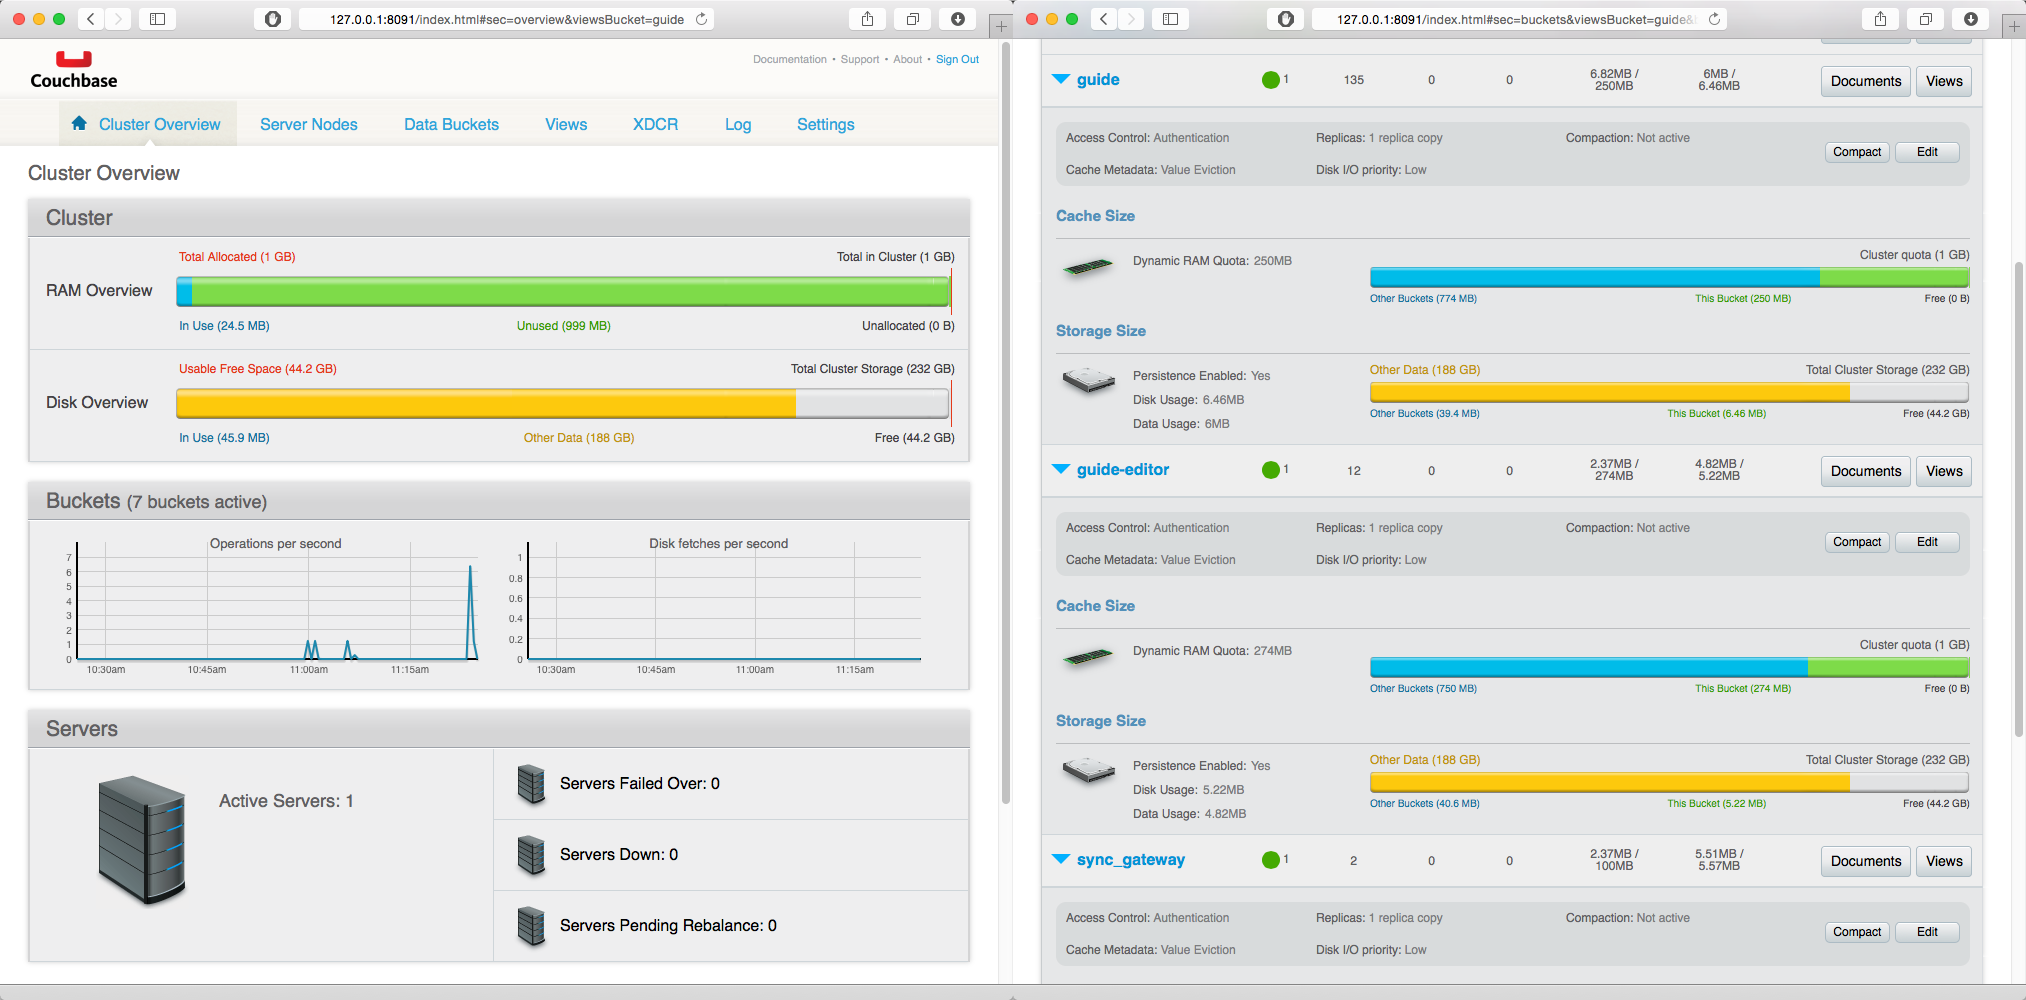
\includegraphics[width=1.0\textwidth]{screen-cbadmin}
\caption{The Couchbase Server management console}
\end{figure}

For the automatic synchronization of the shared bucket between the server and the mobile devices, a "Couchbase Sync Gateway" has to be installed and configured via a json file, where primarily the database server url, the users and the shared bucket are defined.

\begin{lstlisting}[basicstyle=\footnotesize,caption=Connecting the Sync Gateway to the Couchbase Server]
"log": ["HTTP+"],
"databases": {
  "guide": {
    "server": "http://localhost:8091",
    "bucket": "guide",
    "users": {
      "GUEST": {"disabled": false, "admin_channels": ["*"] }
    }
  }
}
\end{lstlisting}

After creating this file and a management bucket named "sync\_gateway" on the server, the gateway can be started and exposes a REST sync API at port 4984 and an admin API at port 4985. A rudimentary synchronization gateway web gui is also available at "localhost:4985/admin/db/guide".

For the shared bucket, all communication has to pass over this synchronization gateway, avoiding to communicate directly to the actual database server. The gateway keeps track of the documents revisions with the management bucket and by adding a management property called "\_sync" to each document, used to save the revision number and other internal version control data. 
